\section{Introduction}
Objects with high-resolution, heterogeneous material properties are everywhere:
from the output of multimaterial 3D printers 
to virtual characters gracing the screen in summer blockbusters.
Designing such objects is made possible by the tight coupling of design
tools and numerical simulation which allows designers 
(or optimization algorithms) to update geometry or material parameters 
and subsequently estimate the physical effects of the change.
Fast, accurate simulation techniques that can handle runtime changes 
in geometry and material composition are a necessity for such iterative design algorithms.
The gold standard technique for estimating the mechanical behavior
of a deformable object under load is the finite element method (FEM).
While accurate, FEM is notoriously slow,
making it a major bottleneck in the iterative design process.
For this reason, there have been a large number of works on speeding up FEM simulations,
and these speed improvements have enabled FEM to be used in many performance critical tasks
such as computer animation, surgical training, and virtual/augmented reality.
Unfortunately, even though techniques such as model reduction or numerical coarsening 
can achieve order-of-magnitude performance increases,
they require expensive precomputation phases, typically on the order of minutes
for large meshes. This precomputation requires knowledge of an object’s 
geometry and material composition a priori,
something that is not known during a design task.
When the user updates the model by changing the geometry or the material distribution,
the preprocessing step must be run again.
Since this step is inside the design loop,
the user cannot get rapid feedback on the changes made to the object.
Additionally, many existing methods assume the object only undergoes small deformations
with known boundary conditions.
Extensions of these methods to large deformations with varying boundary conditions
severely increase the algorithm complexity and quickly diminishes the performance improvements.
\subsection{Coarsening}
We propose coarsening algorithms based on standard FEM
without introducing new types of spatial discretization which increases
algorithmic complexity.
Our algorithm reduces the element count by using coarser elements with data-driven
material properties suitable for design tasks.
The data is acquired before design iterations either from high-resolution simulations or from measurements.
At runtime, precomputed element material properties are applied to a coarse discretization.
The coarsened FEM models can accommodate varying geometry,
material assignments and boundary conditions of an elastic object.
We will fabricate exemplar objects and design physics experiments to validate that our coarsened approximations are sufficiently predictive of object behaviors.
An overview of the pipeline is shown in figure~\ref{fig:overview}.
\begin{figure}[ht]
	\centering
	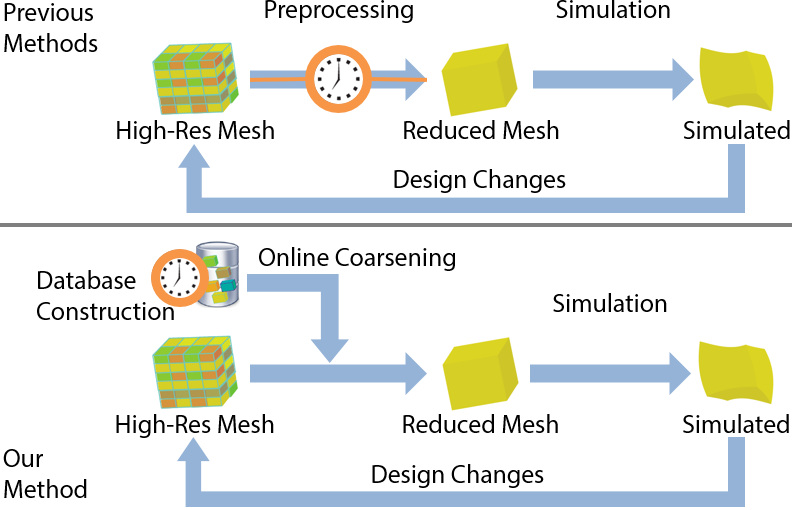
\includegraphics[width=0.7\columnwidth]{images/overview.png}
	\caption{
		In a typical method (top), the preprocessing step of reducing element count is performed for every design change, making the design loop slow.
		In our method (bottom), we move the time-consuming offline computation outside of the design loop.
	}
	\label{fig:overview}
\end{figure}
\subsection{Inverse Design}
Many engineering problems focus on the design of complex structures that needs to meet high level objectives such as the capability to support localized stresses, optimal tradeoffs between compliance and mass, minimal deformation under thermal changes, etc. One very popular approach to design such structures is topology optimization. It computes material distribution over elements to optimize given functional goals \cite{bendsoe2004topology}.
Traditionally, it focused on designs made of homogeneous materials and was concerned with macroscopic changes in the object geometry.
With the advent of multi-material 3D printing techniques, it is now possible to manufacture objects at a much higher resolution, allowing much finer designs and improved functional performances.
Unfortunately, standard techniques for topology optimization do not scale well and they cannot be run on objects with billions of voxels. This is because the number of variables to optimize increases linearly with the number of cells. Since many current 3D printers have a resolution of 600DPI or more, a one billion voxel design occupies only a 1.67 inch cube.

One direction to improve scalability is to work with microstructures corresponding to blocks of voxels instead of individual voxels directly. Recent works followed this direction and proposed to decouple macro structural design and micro material design \cite{rodrigues:2002:hierarchical,coelho:2008:hierarchical,nakshatrala:2013:nonlinear}. However, these approaches remain computationally expensive and, in most cases, limited to the well-known minimal compliance problem.
The second direction to reduce the problem complexity is to temporarily ignore the geometry of the microstructures and consider only their macroscopic physical behavior.
However, this introduces new difficulties as the space of material properties covered by all printable microstructures is much wider than the properties of the base materials.
For example, microstructures made of alternating layers of soft and stiff isotropic materials exhibit an anisotropic behavior as they stretch more easily in one direction than in the others.
This implies that not only the {\it range} but also the complexity of physical behavior of these microstructures increases.
To make use the microstructures in inverse design problems, one needs to solve two challenging problems:
(i) computing the {\it gamut} -- i.e the set -- of the material properties achievable by all microstructures, (ii) efficiently optimizing the distribution of these material properties inside the layout of the object.
\subsection{Microstructure Design}
The material property gamut not only speeds up the inverse design process,
but also allows us to discover families of microstructures with extremal physical properties.
Microstructures can exhibit remarkable physical properties that extend beyond the properties of their constituent materials.
Many microstructure types have been developed to demonstrate applications in mechanics~\cite{milton1995,Kadic2012,Meza2014,Zheng2014,Wang2016Therm,li2016mechanical},
acoustics~\cite{fang2006ultrasonic,li2009experimental},
and electromagnetics~\cite{schurig2006metamaterial,shalaev2007optical,magnus2008dc}.
Microstructures are typically designed manually by domain experts.
These designs are often programmable in the sense that they have a small number of parameters to generate a family of geometries.
A sample set from a given microstructure family can be tested with simulations or experimental measurements.
The mapping between parameters and physical properties helps in gaining insights into the underlying design principles.
In practical applications, it also allows for the selection of a family member that has a desired tradeoff of physical properties~\cite{gibson1982mechanics}.
Unfortunately, it is rare for manually designed microstructure families to reach extremal properties.
This is because the space of possible microstructure designs is combinatorial and therefore impossible to explore exhaustively.
On the other hand, computational methods, such as topology optimization~\cite{sigmund1994materials,sigmund1995tailoring,vogiatzis2017topology},
use a computer simulation in their inner loop to find a microstructure with a desired tradeoff of physical properties.
However, constructing parametric models from optimized structures requires further expertise and manual design effort~\cite{clausen2015topology}.
In contrast to previous work, we propose the first computational method to automatically explore the space of microstructure designs and discover parametric families optimized for competing properties.
